\setcounter{NAT@ctr}{-1}

\phantomsection
\addcontentsline{toc}{section}{The Bio: Virtual Normal}
\articletitle{Discriminating somatic and germline\\mutations in tumor DNA samples without\\matching normals}
Saskia Hiltemann\textsuperscript{\ref{affil:emc-bioinf}},
Guido Jenster\textsuperscript{\ref{affil:emc-urology}},
Jan Trapman\textsuperscript{\ref{affil:emc-pathology}},
Peter van der Spek\textsuperscript{\ref{affil:emc-bioinf}},
Andrew Stubbs\textsuperscript{\ref{affil:emc-bioinf}}

\small
\begin{enumerate}
\itemsep-0.5em
\item Department of Bioinformatics, Erasmus Medical Center, Rotterdam, The Netherlands. \label{affil:emc-bioinf}
\item Department of Urology, Erasmus Medical Center, Rotterdam, The Netherlands \label{affil:emc-urology}
\item Department of Pathology, Erasmus Medical Center, Rotterdam, The Netherlands. \label{affil:emc-pathology}
\end{enumerate}

{\color{chaptergrey}{Published in:}} Genome Research \\
{\color{chaptergrey}{DOI:}} \hyperref[https://doi.org/10.1101/gr.183053.114]{10.1101/gr.183053.114}
% https://link.springer.com/article/10.1007/s10096-018-3220-z

\normalsize

\section*{Abstract}

Tumor analyses commonly employ a correction with a matched normal (MN), a sample from healthy tissue of the same individual, in order to distinguish germline mutations from somatic mutations. Since the majority of variants found in an individual are thought to be common within the population, we constructed a set of 931 samples from healthy, unrelated individuals, originating from two different sequencing platforms, to serve as a virtual normal (VN) in the absence of such an associated normal sample. Our approach removed (1) >96\% of the germline variants also removed by the MN sample and (2) a large number (2\%–8\%) of additional variants not corrected for by the associated normal. The combination of the VN with the MN improved the correction for polymorphisms significantly, with up to ∼30\% compared with MN and ∼15\% compared with VN only. We determined the number of unrelated genomes needed in order to correct at least as efficiently as the MN is about 200 for structural variations (SVs) and about 400 for single-nucleotide variants (SNVs) and indels. In addition, we propose that the removal of common variants with purely position-based methods is inaccurate and incurs additional false-positive somatic variants, and more sophisticated algorithms, which are capable of leveraging information about the area surrounding variants, are needed for optimal accuracy. Our VN correction method can be used to analyze any list of variants, regardless of sequencing platform of origin. This VN methodology is available for use on our public Galaxy server.

\section*{Introduction}

Analysis of 1092 human genomes performed by the 1000 Genomes Project reveals that an individual has approximately 4 million variations (on average, 3.7 million SNPs, 350,000 insertions and deletions [indels], and 750 large deletions) compared with the reference genome and that the vast majority of an individual's germline variations are polymorphic within the human population, with >95\% of all single-nucleotide variants (SNVs) and small indels in a given individual occurring at a frequency of ≥0.5\% (The 1000 Genomes Project Consortium 2010, 2012). Therefore, whenever a matched normal (MN) sample was unavailable (most commonly due to lack of funds or sample availability), researchers have typically relied on the public mutation databases and/or a set of in-house genomes for the filtering of germline variants from the full set of variants found in a tumor sample (Yoon et al. 2009; Kumar et al. 2011). In recent years, these catalogs of human variation have grown exponentially, causing some researchers to question the necessity of sequencing a MN control for every tumor sample (Kumar et al. 2011).

In this study, we address the questions of whether current mutation databases are complete enough to correct for common and rare polymorphisms and of how well this filtering performs compared with the correction with a MN sample.

There are many public databases of human variation available. The Single Nucleotide Polymorphism Database (dbSNP) is a free public archive for genetic variation within and across different species (Sherry et al. 2001). Its latest build (138) contains over 63 million polymorphisms found within the human population. The 1000 Genomes Project (1000G) database contains polymorphisms encountered in a set of 1092 genomes of healthy individuals (The 1000 Genomes Project Consortium 2010, 2012). The NHLBI Exome Variant Server (EVS) contains exonic variants from over 6500 genomes (\url{http://evs.gs.washington.edu/EVS}).

In an effort to improve the control-free correction method further, we constructed what we call a virtual normal (VN). This is a set of 931 samples from healthy, unrelated individuals, whole-genome-sequenced to high depth, originating from two different sequencing platforms. Our VN consists of 433 public samples from Complete Genomics (Drmanac et al. 2010), sequenced in the context of the 1000G, as well as 498 samples sequenced on Illumina HiSeq technology by the Genome of the Netherlands (GoNL) Consortium (Boomsma et al. 2013; The Genome of the Netherlands Consortium 2014).

For copy-number analysis of sequencing data, tools exist that correct for normal contamination in unmatched tumor samples (Boeva et al. 2010). The idea of using a set of genomes for correction of copy-number variants has also been described (Yoon et al. 2009). Apart from a correction based on GC content, this read-depth method also corrects for regions found to have an increased or decreased copy number across all five of their samples (from healthy individuals) and therefore likely a polymorphism within the population. We aim to assess the validity of such an approach and extend it by applying it to structural variation (SV), as well as SNV and indel analysis, in whole-genome-sequenced cancer samples. Additionally, we investigate the minimal size of such a VN necessary for adequate filtering and assess the influence of different ethnicities within the set.

Variants in mutation databases are usually represented only by their position relative to the reference genome and the variant allele, as well as possibly a quality metric. The advantage of using a VN is that we can also leverage information about the area surrounding a variant (e.g., nearby variants in the same sample) to optimize correction. There are often several different ways to describe the same variant, possibly involving (slightly) different chromosomal positions, which means that comparison methods that require an exact match of position and variant nucleotides may be suboptimal, leading to false-positive somatic variants. The algorithm we use with our VN correction is capable of detecting equivalences of differently described variants by taking into account the reference sequence surrounding a variant, as well as neighboring variants. This provides a valuable improvement over correction using variant databases, where this contextual information is lost.

\section*{Results}

We evaluate the performance of the different correction methods on four tumor-normal pairs from two different tumor types (breast and prostate cancer). All of the samples were sequenced by Complete Genomics. Two of the samples were also sequenced using Illumina technology. We evaluate the correction of SNVs and indels of up to ∼50 bp, as well as the larger SVs. For the breast cancer samples, additional validation data were available from the COSMIC database, and we used these confirmed variants to assess the performance of the three different correction methods (MN, mutation databases, VN).

We have made our VN correction method available as a tool for the Galaxy workflow platform (Giardine et al. 2005; Blankenberg et al. 2010; Goecks et al. 2010) as part of our tumor analysis in Galaxy (TAG) tool suite (Hiltemann et al. 2014).

\subsection*{MN vs. VN}

We use three correction methods in order to determine the set of tumor-specific (somatic) variants: a correction for germline variants using a MN sample, a correction for polymorphisms using the VN, and a correction for polymorphisms using public mutation databases (dbSNP, 1000G, and EVS). All variants remaining after application of all three correction methods represent the (consensus) set of true somatic variants. A false-positive variant of a method is any variant remaining after correction, which would have been removed had we employed all three correction methods.

\subsection*{Structural variations}

There are far fewer common SVs, than SNVs and indels, present in public databases. And the few sources of common SVs contain almost exclusively copy-number variants (large indels) and almost none of the more complex SVs such as inversions and translocations. This makes filtering of tumor variants when there is no MN sample very challenging. The Database of Genomic Variants (DGV) (MacDonald et al. 2014) is currently the largest SV database, with approximately 200,000 variants. However, >99\% of these variants are copy-number changes (gains or losses), and the database contains only a limited number of the more complex structural variant types such as inversions and (balanced) translocations, while these are thought to be common in the normal population (Sharp et al. 2006; The 1000 Genomes Project Consortium 2010, 2012; Mills et al. 2011). We additionally filtered using BreakSeq database (Lam et al. 2010), BreakDB (Korbel et al. 2009), and the 1000G SVs (The 1000 Genomes Project Consortium 2010, 2012), which collectively contain another 32,000 structural variants.

We compared the SVs found in the tumor sample to those in the online databases and the VN. We consider two SVs a match if both sides of the event occur within a small distance of the sides of the other SV (200 bp when originating from the same platform, 500 bp when cross-platform).

In the Complete Genomics samples, the VN method removed most of the germline structural variants also removed by the associated normal (∼97\%) while also removing a further 6\%–8\% of common variants not corrected for by the associated normal.

For the Illumina samples, the VN method removed fewer SVs than the MN but was still a huge improvement over using only the database filter. The Illumina HCC1187 sample had 132,045 SVs identified in the tumor sample, of which 1464 were of high quality (QUAL ≥ 200). By use of the VN filter, we removed 961 polymorphic variants from this list (\hyperref[fig:svcomparison]{Fig. \ref{fig:svcomparison}}). Increasing the distance parameter further (to 2000–5000 bp) resulted in the filtering of more SVs than the MN.

\begin{figure}[t!]
\centering
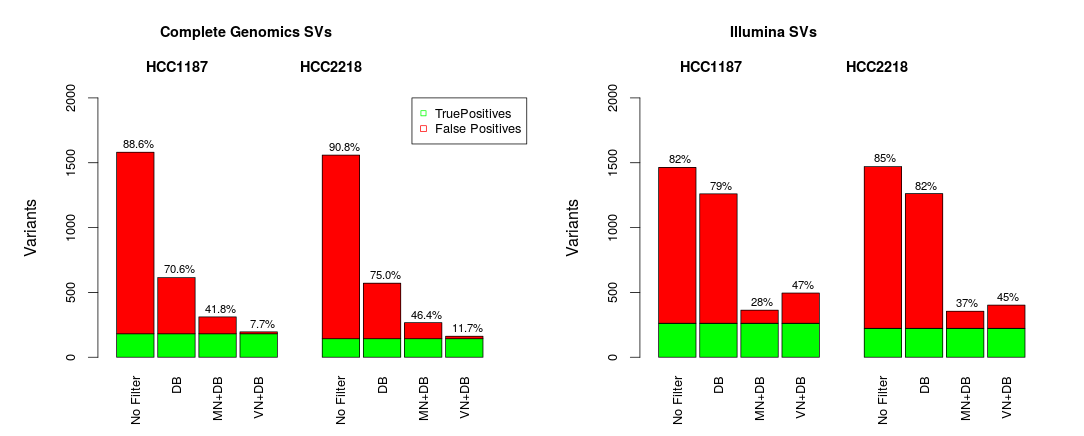
\includegraphics[width=\textwidth]{chapters/images/virtualnormal/Hiltemann_Figure1.png}
\caption{\textbf{Comparison of matched normal (MN) and virtual normal (VN) methods for structural variations (SVs).} Correction of high-confidence SVs from Complete Genomics (left) and Illumina (right), using the database filter (DB), MN, and VN. Light gray area indicates the golden set (combination of the three).}
\label{fig:svcomparison}
\end{figure}

Experimental validation data for the two public genomes HCC1187 and HCC2218 were obtained from the COSMIC database (Forbes et al. 2008, 2011). We determined the number of these confirmed somatic SVs detected in each sample and determined the number of detected SVs that survived our correction method (\hyperref[table:table]{Table \ref{table:table1}}). The CG samples had higher sensitivity (detected more of the validated SVs), but for every tumor sample, those variants that were detected by the platform and determined somatic after correction with the MN all survived correction with VN and DB.

\small
\begin{table}[t!]
\begin{tabular}{lllll}
          & Sample & Detected & Somatic & Description of variants \\
          &        &          &         & called nonsomatic       \\\hline
Illumina  & HCC1187 & 71 of 98 & 53 & 53 of
\end{tabular}
\caption{Number of confirmed somatic SVs (as described in COSMIC database) detected in the tumor samples by CG and Illumina, and the number of these variants that are labeled soatic after corrections with our VN method}
\label{table:table1}
\end{table}
\normalsize

\subsection*{SNVs and indels}




\cite{ireport}


\bibliographystyle{ieeetr}
\bibliography{references}
